\def\year{2022}\relax
%File: formatting-instructions-latex-2022.tex
%release 2022.1
\documentclass[letterpaper]{article} % DO NOT CHANGE THIS
\usepackage{aaai22}  % DO NOT CHANGE THIS
\usepackage{times}  % DO NOT CHANGE THIS
\usepackage{helvet}  % DO NOT CHANGE THIS
\usepackage{courier}  % DO NOT CHANGE THIS
\usepackage[hyphens]{url}  % DO NOT CHANGE THIS
\usepackage{graphicx} % DO NOT CHANGE THIS
\urlstyle{rm} % DO NOT CHANGE THIS
\def\UrlFont{\rm}  % DO NOT CHANGE THIS
\usepackage{natbib}  % DO NOT CHANGE THIS AND DO NOT ADD ANY OPTIONS TO IT
\usepackage{caption} % DO NOT CHANGE THIS AND DO NOT ADD ANY OPTIONS TO IT
\usepackage[shortlabels]{enumitem}
\DeclareCaptionStyle{ruled}{labelfont=normalfont,labelsep=colon,strut=off} % DO NOT CHANGE THIS
\frenchspacing  % DO NOT CHANGE THIS
\setlength{\pdfpagewidth}{8.5in}  % DO NOT CHANGE THIS
\setlength{\pdfpageheight}{11in}  % DO NOT CHANGE THIS

% These are recommended to typeset algorithms but not required. See the subsubsection on algorithms. Remove them if you don't have algorithms in your paper.
% \usepackage{algorithm}
% \usepackage{algorithmic}


% These are are recommended to typeset listings but not required. See the subsubsection on listing. Remove this block if you don't have listings in your paper.
\usepackage{newfloat}
\usepackage{listings}
\lstset{%
	basicstyle={\footnotesize\ttfamily},% footnotesize acceptable for monospace
	numbers=left,numberstyle=\footnotesize,xleftmargin=2em,% show line numbers, remove this entire line if you don't want the numbers.
	aboveskip=0pt,belowskip=0pt,%
	showstringspaces=false,tabsize=2,breaklines=true}
% \floatstyle{ruled}
% \newfloat{listing}{tb}{lst}{}
% \floatname{listing}{Listing}

%\nocopyright

% PDF Info Is REQUIRED.
% For /Title, write your title in Mixed Case.
% Don't use accents or commands. Retain the parentheses.
% For /Author, add all authors within the parentheses,
% separated by commas. No accents, special characters
% or commands are allowed.
% Keep the /TemplateVersion tag as is
\pdfinfo{
/Title (Explainable Shapley-Based Allocation)
/Author (Meir Nizri, Amos Azaria, Noam Hazon)
/TemplateVersion (2022.1)
}


\usepackage[ruled,linesnumbered,vlined]{algorithm2e}
\usepackage{pdfpages}

% Use the postscript times font!
\usepackage{times}
% \usepackage{breqn}
% \usepackage{enumerate}

% \usepackage[utf8]{inputenc}
% \usepackage{comment}
\usepackage{amsmath}
\usepackage{amsthm}
\usepackage{amssymb}
%\usepackage{slashbox}
\usepackage{diagbox}
\usepackage{csquotes}

\newtheorem{theorem}{Theorem}
\newtheorem{corollary}{Corollary}
\newtheorem{lemma}{Lemma}
\newtheorem{observation}{Observation}
\newtheorem{definition}{Definition}
\newtheorem{example}{Example}

\setcounter{secnumdepth}{1} %May be changed to 1 or 2 if section numbers are desired.

\def\set#1{\{#1\}}






\title{Explainable Shapley-Based Allocation}
%  \author{Paper \#5595}
\author {
    % Authors
    Meir Nizri\textsuperscript{\rm 1},
    Amos Azaria\textsuperscript{\rm 1},
    Noam Hazon\textsuperscript{\rm 1}
}
\affiliations {
    % Affiliations
    \textsuperscript{\rm 1} Department of Computer Science\\  Data Science and Artificial Intelligence Center\\ Ariel University, Israel\\
    meir.nizri@msmail.ariel.ac.il, 
    amos.azaria@ariel.ac.il,
    noamh@ariel.ac.il
}

\begin{document}

\maketitle


\begin{abstract}
The Shapley value is one of the most important normative division scheme in cooperative game theory, satisfying basic axioms. However, some allocation according to the Shapley value may seem unfair to humans.
In this paper, we develop an automatic method that generates intuitive explanations for a Shapley-based payoff allocation, which utilizes the basic axioms.
Given a coalitional game, our method decomposes it to sub-games, for which it is easy to generate verbal explanations, and shows that the given game is composed of the sub-games. 
Since the payoff allocation for each sub-game is perceived as fair, the Shapley-based payoff allocation for the given game should seem fair as well.
We run an experiment with $210$ human participants and show that when applying our method, humans perceive Shapley-based payoff allocation as significantly more fair than when using a general standard explanation.
\end{abstract}


%{\bf Keywords:} Shapley Value; Explainable AI; Human Perception; Fair Division  % put your semicolon-separated keywords here!


\section{Introduction}

The Shapley value \cite{shapley1953value}, which has been termed the most important normative division scheme in cooperative game theory \cite{winter2002shapley},
is based on the idea that the payoff of the game should be divided such that each agent’s share is proportional to its contribution to the payoff. 
%Specifically, the Shapley value is the average expected marginal contribution of one agent to all possible subsets of agents. 
Indeed, the Shapley value is considered fair since it is the only payoff allocation that satisfies the following four desirable axioms: efficiency, symmetry, null player property and additivity \cite{hart1989shapley}. %(see Section \ref{sec:defn} for formal definitions).
%These axioms admit strong normative and positive interpretations \cite{de2018membership}.

%It may seem unfair at times
While the axioms satisfied by the Shapley value seem necessary, humans presented with an allocation according to the Shapley value may sometimes not observe it as fair. For example, consider the following game with three agents: $r$, $l_1$, and $l_2$, which is also known as the classical ``glove game''. Agents $l_1$ and $l_2$ have a left-glove and agent $r$ has a right-glove. A pair of left and right gloves is worth $\$12$, but a single glove is worth nothing. If all agents collaborate, the Shapley value allocates $\$8$ to agent $r$ and only $\$2$ to $l_1$ and $\$2$ to $l_2$. While it seems plausible that agent $r$ should receive a higher payoff, a right-glove alone is worth nothing and thus, it may seem unfair that the payoff for this agent is $4$-times more than each of the other agents. However, any other allocation would violate at least one of the axioms. It is thus desirable to increase human acceptance of the allocation according to the Shapley value, which can be achieved by providing explanations. 
In this paper, we develop an automatic method that generates intuitive explanations for a Shapley-based payoff allocation.

%We build upon the three principles of the Shapley value
% There are many possible ways for generating explanations for a Shapley-based payoff allocation. Indeed, Procaccia claimed that ``the central role of axioms should be to help explain the mechanism’s outcomes to participants'' \cite{procaccia2019axioms}, and this direction has been successfully applied in the field of fair division by the \textit{Spliddit} website\footnote{\url{http://www.spliddit.org/}} \cite{Goldman14spliddit:unleashing}. We follow this idea, and build our explanations on top of the four axioms of the Shapley value. 
% which are the following.
% \textit{Efficiency} requires that the sum of all agents payoff equals the amount obtained when all agents collaborate. 
% \textit{Symmetry} states that if two agents are equivalent, i.e., they contribute equally to each coalition, their payoff should be equal. The \textit{null-player} axiom requires that any agent that does not contribute to any coalition, would have a payoff of $0$. Finally, the \textit{additivity} axiom states that if a new game is obtained by adding two different games with the same set of agents, the payoff of an agent in the new game is equal to the sum of its allocation in the two games separately. 
% We note that there are several equivalent sets of axioms that characterize the Shapley value \cite{moulin2004fair}.
%Efficiency, symmetry, and null player are properties of a single game, while additivity is a property of multiple games.

Now, the essence of our explanation is that any game is decomposed into several sub-games that their Shapley allocation is easier to perceive as fair. Specifically, any sub-games is built such that all the agents are either null players or equivalent to one another, and the values are either all non-negative or all non-positive.
According to the null player axiom each agent who is a null player should receive a payoff of $0$, and according to the symmetry and efficiency axioms all other agents should equally share the total outcome, and thus the Shapley allocation in each sub-game is intuitively fair.
For example, the ``glove game'' can be decomposed into few sub-games; in one of the sub-games, agent $r$ obtains a value of $\$12$ when collaborating with $l_1$, but not when collaborating with $l_2$. When all three agents collaborate, they obtain a value of $\$12$. In this sub-game $l_2$ is a null player, and agents $r$ and $l_1$ are equivalent. Thus, the Shapley allocation of $\$6$ to agent $r$, $\$6$ to agent $l_1$ and $\$0$ to agent $l_2$ is intuitively fair. Finally, following the additivity axiom, since the Shapley allocation of every sub-game is intuitively fair, and the sum of the Shapley allocations in each sub-game is equal to the Shapley allocation in the original game, then the latter is easier to perceive as fair. We note that this process follows the arguments in the proof of the uniqueness of the Shapley value \cite{shapley1953value}.
Practically, we do not directly present the axioms to the users. Instead, our algorithm, which we termed \textit{X-SHAP}, decomposes any coalitional game into several sub-games, and automatically generates a brief verbal explanation that accompanies each sub-game.
% For example, recall the sub-game of the ``glove game'' that we have previously mentioned. X-SHAP presents the sub-game to the user, and generates the following verbal explanation: 
% \begin{displayquote}
% \textit{``In this scenario, $l_2$ does not contribute anything. $r$ and $l_1$ are identical and always contribute the same. Therefore, the total revenue, which is $\$12$, should be equally divided between $r$ and $l_1$, and thus, the fair division is $r:\$6, l_1:\$6, l_2:\$0$.'' }
% \end{displayquote}
% Similarly, X-SHAP presents the other sub-games along with their explanations.
% X-SHAP finalizes its explanation by stressing out that since the sum of all the sub-games is the original game, the proposed division is fair as it is the sum of all the sub-games divisions.


We run an experiment with $210$ human participants and show that %when applying our method, humans perceive Shapley-based payoff allocation as significantly more fair than when using a general standard explanation.
the explanations that were generated by X-SHAP achieved significantly higher fairness rating compared to the general explanation in all the games examined. This indicates that humans perceive the Shapley payoff allocation fairer if they receive X-SHAP's explanations.

To summarize, the main contribution of this paper is that it provides the first successful automatic method that generates customized explanations of the Shapley allocation for any given coalitional game.



\subsection{Related Work}
Our work belongs to the field of Explainable AI (XAI) \cite{gunning2019xai}. %In a typical XAI setting, the goal is to explain the output of an AI system to a human. This explanation is important for allowing the human to trust the system, better understand, and to allow transparency of the system's output \cite{adadi2018peeking}. Other XAI systems are designed to provide explanations, comprehensible by humans, for legal or ethical reasons \cite{doran2017does}. For example, an AI system for the medical domain might be required to explain its choice for recommending the prescription of a specific drug \cite{holzinger2017need}. Indeed, most of the work on XAI concerned with the explanation of a machine learning based model. In this paper, we develop a system for explaining a solution concept that is based on a set of axioms.
%Our work can be also seen as an instance of x-MASE \cite{kraus2020ai}, explainable decisions in multiagent environments.
%
The work that is closest to ours is the paper by Cailloux and Endriss \cite{Cailloux2016ArguingAV}. 
%They propose a logic-based system for providing justifications for the outcome of a voting rule.
They %also
develop an algorithm that automatically derives a justification for any outcome of the Borda rule. The algorithm's main idea is to decompose the preference profile into a sequence of sub-profiles, and use one of six axioms for providing explanations for the sub-profiles and for their combinations. %This approach is further extended by
% \cite{peters2020explainable}, which investigate the required length of the sequence of explanations.
Our approach for explaining the Shapley allocation is also based on axioms, and we also decompose the given coalitional game into a set of sub-games, which together compose an explanation for the given coalitional game.  

% Another work that analyzes a decomposition of a coalitional game in relation with the Shapley value is the paper by Stern and Tettenhorst \shortcite{stern2019hodge}. They provide a new characterization of the Shapley value, by showing that a coalitional game can be decomposed into sub-games, one sub-game for each agent. They prove that the Shapley value equals the value of the grand coalition in each agent's sub-game \cite{stern2019hodge}.
% Similarly, \cite{de2018membership} provides a new axiomatization for the Shapley value by replacing the additivity axiom with the difference formula (DF) axiom. The DF axiom requires that each agent's payoff can be obtained by subtracting two functions: one function depending on the values of all sets that the agent belongs to, and the other depending on those that she does not belong to.

Spliddit \cite{Goldman14spliddit:unleashing} is a website implementing algorithms for various division tasks (e.g., rent division), which also explains how the outcomes satisfy certain fairness requisites.
While the website enables users to compute the Shapley value in a ride-sharing context, it provides only a general explanation that states the benefits of the Shapley value. 
Our work can thus serve as an extension for Spliddit by providing customized explanations for the Shapley value.

% The Shapley value can also be applied for increasing interoperability of a machine learning model. For example, Lundberg and Lee \shortcite{lundberg2017unified} 
% provide explanations based on quantifying the importance of the features by applying the Shapley value. In their setting, the features are considered as agents and the value for every subset of features is the accuracy of the model when only those features are used. 





\section{X-SHAP}
In this section we propose the \textit{X-SHAP} algorithm, % (Algorithm \ref{alg:xshap}),
which given any coalitional game, automatically decomposes the coalitional game into a number of sub-games. %along with their explanation.
% Given the ETX sub-games, X-SHAP automatically generates explanations for each of them (as described in Section \ref{sec:etx}) and presents the payoff allocations along with the explanations to human users. It is expected that humans will find the Shapley value payoff to be fair in each of the ETX sub-games, and thus the Shapley value for the given game, which is composed of the sub-games, should seem fair to humans as well.

The \textit{X-SHAP} algorithm works as follows. It receives a coalitional game $(N,v)$ as an input and provides a set $X$ of characteristic functions that maintains the following two properties:
\begin{enumerate}
\item Each coalitional game $(N,x)$, where $x \in X$, is easy-to-explain.
\item The sum of all the characteristic functions in $X$ equals $v$. That is, $\sum_{x \in X} x = v$.
\end{enumerate}
Note that since the Shapley value satisfies the additivity axiom, the sum of Shapley value payoffs assigned to each agent $i \in N$ in each characteristic function in $X$ is equal to the Shapley value payoff for $i$ in $(N,v)$. That is, $\forall i \in N, \sum_{x \in X} Sh_i (N, x) = Sh_i (N, v)$. Once the set $X$ is generated, we generate explanations for each of the sub-games.

Algorithm~\ref{alg:xshap} describes the pseudo-code for \textit{X-SHAP}.
The algorithm iterates over all subsets $S \subseteq N$ in ascending order according to $|S|$. It maintains a characteristic function $accum$ that accumulates all the characteristic functions it builds in each iteration.
For each subset $S$ whose value in $v$ is different from its value in $accum$, X-SHAP adds the following characteristic function $x$ to $X$. For each subset of $N$, $T$, that contains $S$, $x(T)$ is set to the difference between $v(S)$ and $accum(S)$. 

\begin{algorithm} [hbpt]
\caption{X-SHAP}
\label{alg:xshap}
\SetKwInOut{Input}{Input}
\SetKwInOut{Output}{Output}
    \Input{A coalitional game $(N, v)$.}
    \Output{A set of characteristic functions $X$, along with their explanations.}
    $X \gets \emptyset$\\
    Let $accum, x$ be characteristic functions on $N$\\
    Initialize $accum$ to $0$ for any subset\\
    \For{$i\gets 1$ to $|N|$} {
        \For{every $S \subseteq N$, such that $|S|=i$} {
            Initialize $x$ to $0$ for any subset\\
            \If{$v(S) \neq accum(S)$}{
                \For{every $T \supseteq  S$} {
                    $x(T) \gets v(S) - accum(S)$ \label{line:update_x}
                }
                $X \gets X \cup \set{x}$\\
                $accum \gets accum + x$ \label{line:update_accum}
            }
        }
    }
    Generate an explanation for each $x\in X$ \\
    \Return $X$ along with the explanations\\
\end{algorithm}

% The number of characteristic functions in $X$ is at most the number of subsets in $N$, which is $2^{|N|}$. 
% Denote $M=2^{|N|}$ and $n=|N|$. A naive implementation of X-SHAP is $O(M^2)$; however, by using the following approach, we can reduce the complexity to $O(M^{\log_23})\approx O(M^{1.58})$. For every subset $S \subseteq N$ we can get all its supersets $T \supseteq S$ by adding $S$ to every subset of $N \setminus S$. %The access to each subset $T \supseteq  S$ is in $O(1)$.
% Now, the number of subsets with $i$ agents is $\binom{n}{i}$, and the number of supersets of every such subset is $2^{n-i}$. Hence, the complexity of X-SHAP is:
% $$\begin{aligned}
% \sum_{i=1}^{n} \binom{n}{i} 2^{n-i} &= \sum_{i=1}^{n} \binom{n}{n-i} 2^{n-i} =
% \sum_{k=0}^{n-1} \binom{n}{k} 2^{k} \\ &=
% \sum_{k=0}^{n} \binom{n}{k} 2^{k} 1^{n-k} - 2^n.
% \end{aligned}$$
% According to the binomial expansion formula, $(x+y)^n = \sum_{k=0}^n \binom{n}{k}x^{k}y^{n-k}$, and thus,
% $$\begin{aligned}
% \sum_{k=0}^{n} \binom{n}{k} 2^{k} 1^{n-k} - 2^n &= (2+1)^n-M = 3^n - M \\ = 3^{\log_2M} -M & = O(M^{\log_23}).
% \end{aligned}$$

% example
% Consider the following example, which illustrates the output that is generated by the X-SHAP algorithm.
% \begin{example}
% Consider the following coalitional game $(N, v)$, in which $N = \set{a,b,c}$, and $v$ associates to every subset of $N$ the following values:
% \begin{center}
% \begin{tabular}{ l|c } 
%  $\set{a}$     & 0    \\ 
%  $\set{b}$     & 0    \\ 
%  $\set{c}$     & 100  \\ 
%  $\set{a,b}$   & 300  \\ 
%  $\set{a,c}$   & 200  \\ 
%  $\set{b,c}$   & 100  \\ 
%  $\set{a,b,c}$ & 500  \\ 
% \end{tabular}
% \end{center}
% The Shapley payoff allocation for each of the agents in this game is $Sh_a(N,v)=200, Sh_b(N,v)=150$ and $Sh_c(N,v)=150$. It is not intuitive that this payoff allocation is indeed fair.
% For this input, X-SHAP outputs a set $X$ with the following characteristic functions:
% \begin{center}
% \begin{tabular}{ l|c c c } 
%  Coalition & (1) & (2) & (3)  \\
%  \hline
%  $\set{a}$     & 0   & 0   & 0     \\ 
%  $\set{b}$     & 0   & 0   & 0     \\ 
%  $\set{c}$     & 100 & 0   & 0     \\ 
%  $\set{a,b}$   & 0   & 300 & 0     \\ 
%  $\set{a,c}$   & 100 & 0   & 100   \\ 
%  $\set{b,c}$   & 100 & 0   & 0     \\ 
%  $\set{a,b,c}$ & 100 & 300 & 100   \\ 
% \end{tabular}
% \end{center}
% Each of these functions is ETX and their sum equals $v$, i.e., $\sum_{x \in X} x = v$. The Shapley payoff allocation for each of the coalitional games $(N,x)$, where $x \in X$ is:
% \begin{center}
% \begin{tabular}{ l|c c c } 
%  Agent & (1) & (2) & (3)  \\
%  \hline
%  $Sh_a$     & 0   & 150  & 50   \\ 
%  $Sh_b$     & 0   & 150  & 0    \\ 
%  $Sh_c$     & 100 & 0    & 50   \\ 
% \end{tabular}
% \end{center}
% In addition, X-SHAP provides the following explanations for each sub-game:
% \begin{enumerate}[(1)]
% \item ``In this scenario, $a$ and $b$ do not contribute anything. The entire revenue is contributed by $c$ alone. Therefore, the total revenue, which is $\$100$, should solely go to $c$, and thus, the fair division is $a:\$0, b:\$0, c:\$100$.''
% \item ``In this scenario, $c$ does not contribute anything. $a$ and $b$ are identical and always contribute the same. Therefore, the total revenue, which is $\$300$, should be equally divided between $a$ and $b$, and thus, the fair division is $a:\$150, b:\$150, c:\$0$.''
% \item ``In this scenario, $b$ does not contribute anything. $a$ and $c$ are identical and always contribute the same. Therefore, the total revenue, which is $\$100$, should be equally divided between $a$ and $c$, and thus, the fair division is $a:\$50, b:\$0, c:\$50$.''
% \end{enumerate}
% Given these payoff allocations and their explanations, it is quite likely that human users will accept each of them as fair. %: in game (1) agent $c$ is responsible for the entire value in any coalition with a value greater than 0. In game (2) agents $a$ and $b$ equally contribute to the entire value, and in game (3) agents $a$ and $c$ equally contribute to the entire value.
% The sum of all the payoff allocations of each agent is indeed equal to the shapely value of the original game $(N,v)$, i.e. $\forall i \in N, \sum_{x \in X} Sh_i (N, x) = Sh_i (N, v)$.\\
% \end{example}


% %\subsection{X-SHAP properties}
% We now prove that the set $X$ of characteristic functions that is returned by Algorithm~\ref{alg:xshap} maintains the required properties.

% \begin{theorem}
% Each coalitional game $(N,x)$, where $x \in X$, is easy-to-explain.
% \end{theorem}
% \begin{proof}
% Given a characteristic function $x \in X$, it corresponds to a subset $S \subseteq N$. X-SHAP constructs $x$ such that it assigns a non-zero value, $val$, for every $T \supseteq S$, and a zero value otherwise. Therefore, for any agent $i \notin S$ and for every subset $P \subseteq N\setminus\set{i}$, it holds that $x(P\cup\set{i}) = x(P)$. That is, every agent $i \notin S$ is a null player.
% On the other hand, every agent $i \in S$ is not a null player, since $x(S \setminus \set{i})=0$ but $x(S) = val \neq 0$.
% In addition, for every two agents $i,j \in S$ and any subset $P \subseteq N\setminus\set{i,j}$, it holds that $x(P\cup\set{i}) = x(P\cup\set{j})$. That is, every two agents $i,j \in S$ are equivalent. Therefore, the coalitional game $(N, x)$ is ETD.
% Finally, for every pair of disjoint subsets $P_1,P_2$, these are the possible cases: \begin{itemize}
%     \item $P_1, P_2 \nsupseteq S$, and thus $v(P_1)=v(P_2)=0$. Now, if $val$ is positive then $v(P_1 \cup P_2) \geq v(P_1)+v(P_2)$, and if $val$ is negative then $v(P_1 \cup P_2) \leq v(P1)+v(P2)$.
%     \item Without loss of generality, $P_1 \supseteq S$ but $P_2 \nsupseteq S$. We get that  $v(P_1)=val$ but $v(P_2)=0$. In addition, since $P_1 \cup P_2 \supseteq S$, $v(P_1 \cup P_2) = val = v(P_1)+v(P_2)$.
% \end{itemize}
% Therefore, if $val$ is positive then $x$ is super-additive and if $val$ is negative then $x$ is sub-additive. That is, $(N, x)$ is clean, and since $(N, x)$ is also ETD it is ETX.
% \end{proof}


% \begin{theorem}
% The sum of all the characteristic functions in $X$ equals $v$. That is, $\sum_{x \in X} x = v$.
% \end{theorem}
% \begin{proof}
% The algorithm iterates over all $S \subseteq N$. At the end of an iteration in which $S \subseteq N$ is considered, $accum(S)$ equals $v(S)$. This is because either $accum(S)$ already equals $v(S)$ or $x(S)$ is set to $v(S)-accum(S)$ in line \ref{line:update_x}, and after line \ref{line:update_accum} $accum(S)$ becomes $v(S)$. After considering $S$ the algorithm does not consider any $S' \subseteq S$, and thus all following iterations do not change $accum(S)$. Finally, according to the algorithm construction, $accum$ holds the sum of all the functions $x \in X$ when the algorithm terminates. Hence, $\sum_{x \in X} x = accum = v$.
% \end{proof}


% note that we sometimes need to use negative values, which correspond to costs allocation
% We note that a characteristic function $x \in X$, that correspond to some coalition $S \subseteq N$, may contain negative values even if $v$ consists of only non-negative values. This situation will occur when the sum of all the characteristic functions constructed before $x$ is higher than $v(S)$. We show that any procedure that decomposes a coalitional game with a non-negative characteristic function into a number of ETX sub-games, cannot avoid using sub-games with a negative characteristic function.

%prove that it cannot be done without negative.
% \begin{theorem}
% There exist coalitional games with non-negative characteristic functions such that any decomposition into ETX sub-games results in at least one sub-game with negative characteristic function.
% \label{theorem:negative}
% \end{theorem}
% \begin{proof}
% Consider the following coalitional game $(N, v)$, which is the classical ``glove game", in which $N = \set{a,b,c}$ and for every $S \subseteq N$, 
% $$v(S)= \begin{cases} 
%         1 & S \in \set{\set{a,b}, \set{a,c}, \set{a,b,c}}\\
%         0 & else. 
%       \end{cases}$$
% Assume towards contradiction that $(N,v)$ can be decomposed into ETX sub-games, such that none of their characteristic functions consist of negative values. Let $X$ be the set of these characteristic functions, and let $X^+_S \subseteq X$, where $S \subseteq N$, be the set of all the characteristic functions in $X$ that assign a value greater than 0 for the coalition $S$. That is, for each $x \in X^+_S$, $x(S)>0$. 
% Since $\sum_{x \in X} x(\set{a,b}) = v(\set{a,b})=1$, and every $x \in X$ does not consist of negative values, it should hold that $\sum_{x \in X^+_{\set{a,b}}} x(\set{a, b}) = 1$. Since each $x \in X^+_{\set{a,b}}$ does not consist of negative values and each sub-game is clean, then by definition $x$ is super-additive; therefore, $\sum_{x \in X^+_{\set{a,b}}} x(\set{a, b, c}) \geq 1$. Furthermore, since $v(\set{a, b, c}) = 1$ and $x$ is non-negative, it must hold that $\sum_{x \in X^+_{\set{a,b}}} x(\set{a, b, c}) = 1$. Similarly, for the set $X^+_{\set{a,c}}$, $\sum_{x \in X^+_{\set{a,c}}} x(\set{a, b, c}) = 1$.

% Now, for any $x \in X^+_{\set{a,b}}$ it must hold that $x \in X^+_{\set{a,c}}$, otherwise, if there is $x' \in X^+_{\set{a,b}}$ such that $x'(\set{a,c})=0$ then $\sum_{x \in X^+_{\set{a,c}}} x(\set{a,b,c}) + x'(\set{a,b,c}) > 1$. Finally, since $v(\set{a}) = v(\set{b}) = v(\set{b,c}) = 0$ and every $x \in X^+_{\set{a,b}}$ is non-negative, $x(\set{a}) = x(\set{b}) = x(\set{b,c}) = 0$. However, $x(\set{a,b})>0$ and thus $a$ and $b$ are not null players in the sub-game $(N,x)$, but  $x(\set{c} \cup \set{a}) = x(\set{a,c}) > 0$ and $x(\set{c} \cup \set{b}) = x(\set{b,c}) = 0$. That is, $a$ and $b$ are not equivalent and thus the sub-game $(N,x)$ is not ETX, which is a contradiction.
% \end{proof}



\section{Experimental Evaluation}
%We show that it works
In order to evaluate the performance of X-SHAP, we conducted a survey with human participants. The survey examined six coalitional games, representing a variety of scenarios. Each of the coalitional games was presented to the participants along with its Shapley payoff allocation as a suggestion for dividing the payoff among the agents. Then, each participant was given either  X-SHAP's explanation or a general explanation that states the benefits of the Shapley value, which served as a baseline. The participants were asked to rate the proposed allocation by indicating to what extent they agree or disagree that it is fair, using a seven-point Likert scale. Overall, 210 different people participated in the survey, each answering two different coalitional games. %Each of the six games was presented to 70 people, with half of them seeing the X-SHAP explanation and the other half seeing the general explanation. 
% In order to evaluate the explanation generated by X-SHAP, we run a survey on Mechanical Turk. The participants were first given an appropriate background on coalitional games in general and instructions specific to the survey. 
% The participants were presented with a coalitional game in which the agents were referred to as entities, and the values of the characteristic function were referred to as revenues. The game was composed of three entities, marked as $a,b,c$, and the participants were presented with a table of revenues of the entities when they are alone and when they collaborate with each other.
% The participants were also presented with the Shapley payoff allocation as a suggestion for dividing the revenue among the three entities when they all collaborate.

% Then, each participant was given either the X-SHAP's explanation specific for the game or a general explanation of the Shapley value, which served as a baseline. 
% Participants were able to switch between all the sub-games so that they can examine each sub-game individually. For each sub-game they were presented with its allocation according to the Shapley value with a brief explanation. Finally, each participant was shown how the sum of all the sub-games and their Shapley value allocation equal to the original game and its Shapley value. 
% % The general explanation was taken from the \textit{Spliddit} website \cite{Goldman14spliddit:unleashing}; it states that the allocation is based on the marginal contribution of each agent to each possible coalition.

% % \begin{figure}[hbpt]
% %     \centering
% %     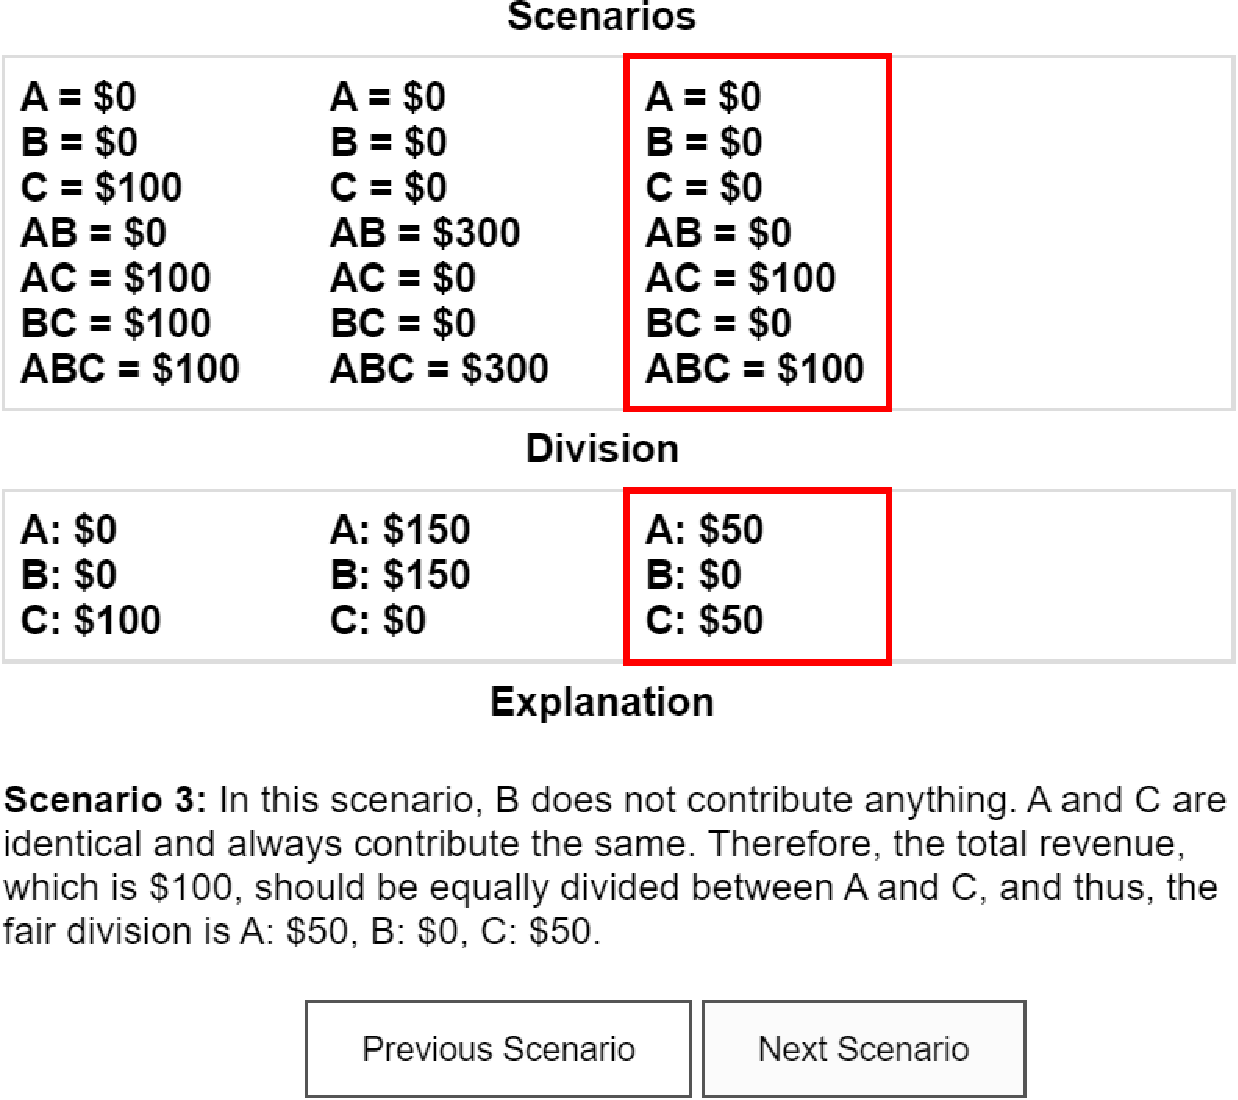
\includegraphics[width=3.3in]{SurveyExample1.pdf}
% %     \caption{Screenshot from the survey of the X-SHAP explanation.}
% %     \label{fig:SurveyExample1}
% % \end{figure}

% %\begin{figure}[hbpt]
% %    \centering
% %    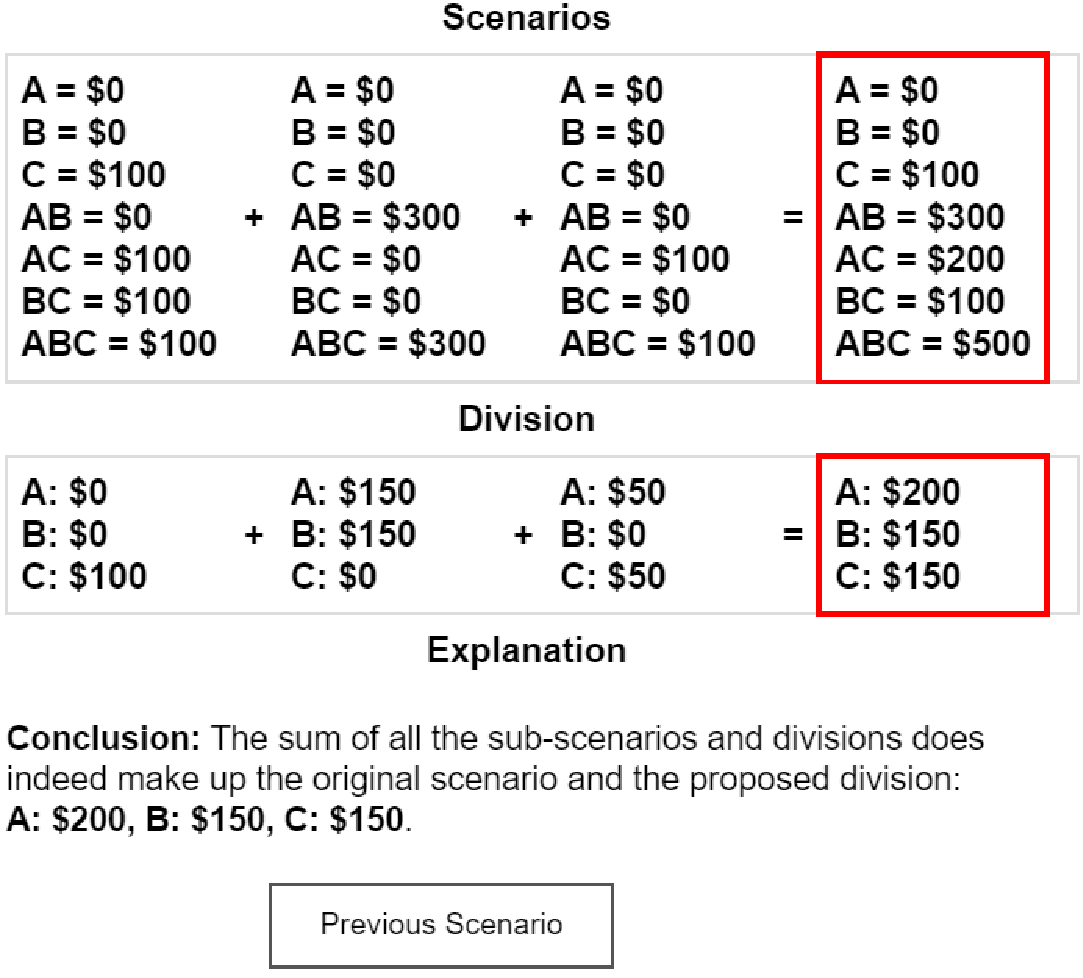
\includegraphics[width=3.3in]{SurveyExample2.pdf}
% %    \caption{Screenshot from the survey of the X-SHAP explanation.}
% %    \label{fig:SurveyExample2}
% %\end{figure}

% The participants were asked to rate the proposed payoff allocation by indicating to what extent they agree or disagree that it is fair. 
% %Likert scale is commonly used in research and surveys to measure attitude, providing a range of responses to a given question or statement. The typical Likert scale is a 5- or a 7-point ordinal scale used by participants to rate the degree to which they agree or disagree with a question or a statement. Therefore, we opt to use a 5-Likert scale
% The participants could choose one of seven options on a Likert scale, between `strongly agree' (7) to `strongly disagree' (1), with the middle being `neither agree nor disagree' (4).

% The participants were then presented with a different coalitional game along with its Shapley payoff allocation. Participants that were shown the X-SHAP explanation for the first coalitional game were given the general explanation for the second game, and vice versa.

% Table~\ref{tbl:games} specifies the coalitional games that we used for the survey. In each of these games $(N,v)$, $N=\set{a,b,c}$, and all revenues are non-negative. The Shapley payoff allocation for each of the scenarios appears in Table \ref{tbl:shap}.

% \begin{table}[hbpt]
% \begin{center}
% \begin{tabular}{ l|c c c c c c} 
%  Coalition & (1) & (2) & (3) & (4) & (5) & (6) \\
%  \hline
%  $\set{a}$     & 200 & 0   & 0   & 0   & 100  &   300  \\
%  $\set{b}$     & 200 & 100 & 0   & 0   & 200  &   0    \\
%  $\set{c}$     & 100 & 200 & 100 & 0   & 300  &   500  \\
%  $\set{a,b}$   & 400 & 300 & 300 & 300 & 200  &   500  \\
%  $\set{a,c}$   & 600 & 400 & 200 & 300 & 300  &   100  \\
%  $\set{b,c}$   & 600 & 300 & 100 & 0   & 300  &   200  \\
%  $\set{a,b,c}$ & 800 & 700 & 500 & 300 & 350  &   600  \\
% \end{tabular}
% \caption{The coalitional games that we used for the survey.}
% \label{tbl:games}
% \end{center}
% \end{table} 
%
% \begin{table}[hbpt]
% \begin{center}
% \begin{tabular}{ l|c c c c c c}
%  Agent & (1) & (2) & (3) & (4) & (5) & (6) \\
%  \hline
%  $Sh_a$     & 250 & 200 & 200 & 200 & 50  & 250 \\
%  $Sh_b$     & 250 & 200 & 150 & 50  & 100 & 150 \\
%  $Sh_c$     & 300 & 300 & 150 & 50  & 200 & 200 \\
% \end{tabular}
% \caption{The Shapley payoff allocation for each of the scenarios from Table \ref{tbl:games}.}
% \label{tbl:shap}
% \end{center}
% \end{table} 

% We chose these coalitional games as they represent a variety of scenarios: in game (1) all the values are greater than zero, and agents $a$ and $b$ are equivalent. In game (2) the value of $\set{a}$ is zero and $a$ and $b$ are not equivalent, but the Shapley payoff for $a$ and $b$ is nevertheless identical. In game (3) the value of $\set{a}$ and $\set{b}$ is zero, there are no equivalent agents, but the Shapley payoff for $b$ and $c$ is nevertheless identical. In game (4) the value of $\set{a}$, $\set{b}$ and $\set{c}$ is zero, yet only $b$ and $c$ are equivalent agents. Note also that game (4) is the glove game mentioned above. The characteristic functions in games (1)-(4) are super-additive. This attribute is common since if two (or more) agents collaborate, they are expected to gain more than each would have gained by herself. Yet, we also tested two less common scenarios:
% In game (5) the characteristic function is sub-additive, while in game (6) the characteristic function is neither super-additive nor sub-additive. 




%Mechanical Turk settings 
%We set a requirement on Mechanical Turk that the approval rate of the works must be at least $99\%$ and did not require the Turkers to be masters. 
%Overall, 210 different people participated in the survey, each answering two different scenarios. We presented six different scenarios, each presented to 70 people, with half of them seeing the X-SHAP explanation and the other half seeing the general explanation. %The average age of the participants is 37 with 117 males and 88 females. Five participants chose not to specify their gender.



%\section{Results}
%Figure~\ref{fig:comparingResult} presents the results. 
The results were obtained by averaging over the 35 ratings of each of the two explanations in each of the six scenarios. The explanations that were generated by X-SHAP significantly outperformed the general explanation in terms of fairness rating in all the scenarios examined ($p<0.0001)$. That is, the human participants perceive the payoff allocation fairer if they receive the explanations that are generated by X-SHAP. Overall, the average fairness rating in scenarios in which the X-SHAP explanation was provided is $5.3$, which is significantly higher than the rating of $4.4$ obtained for scenarios accompanied by the general explanation.

%For checking the statistical significance, we ran an analysis of variance (ANOVA) test, which considers both the scenario and the type of explanation. The ANOVA test yielded $p < 0.0001$. Indeed, analyzing the outcomes of the Likert scale, and the use of parametric tests to analyze ordinal data in general, has been subject to an active and ongoing debate \cite{MUALLA2021103573}. We thus conducted also a non-parametric test, an ordinal logistic regression analysis, which is used to assess the difference between two methods with ordinal values, such as ratings and pain level reporting \cite{harrell2015ordinal}. The ordinal logistic regression analysis also demonstrated the significance of the results ($p < 0.0001$).  
%on the results,  % 3.059E-09$.

% We note that the explanations that were generated by X-SHAP for scenarios (4)-(6) yielded a lower average of fairness rating compared to the explanations for scenarios (1)-(3). A possible reason is that 
% while scenarios (1)-(3) include only characteristic functions with positive values in scenarios (4)-(6) the explanations include characteristic functions with positive values along with characteristic functions with negative values. The combination of positive and negative characteristic functions in one explanation may be confusing. However, this phenomenon cannot be avoided according to theorem \ref{theorem:negative}.
% We also note that Scenario (6) has the lowest average fairness rating for both X-SHAP and the general explanation. A possible reason is that its characteristic function is neither super-additive nor sub-additive, and thus, represents a less intuitive scenario.


% \begin{figure}[hbpt]
%     \centering
%     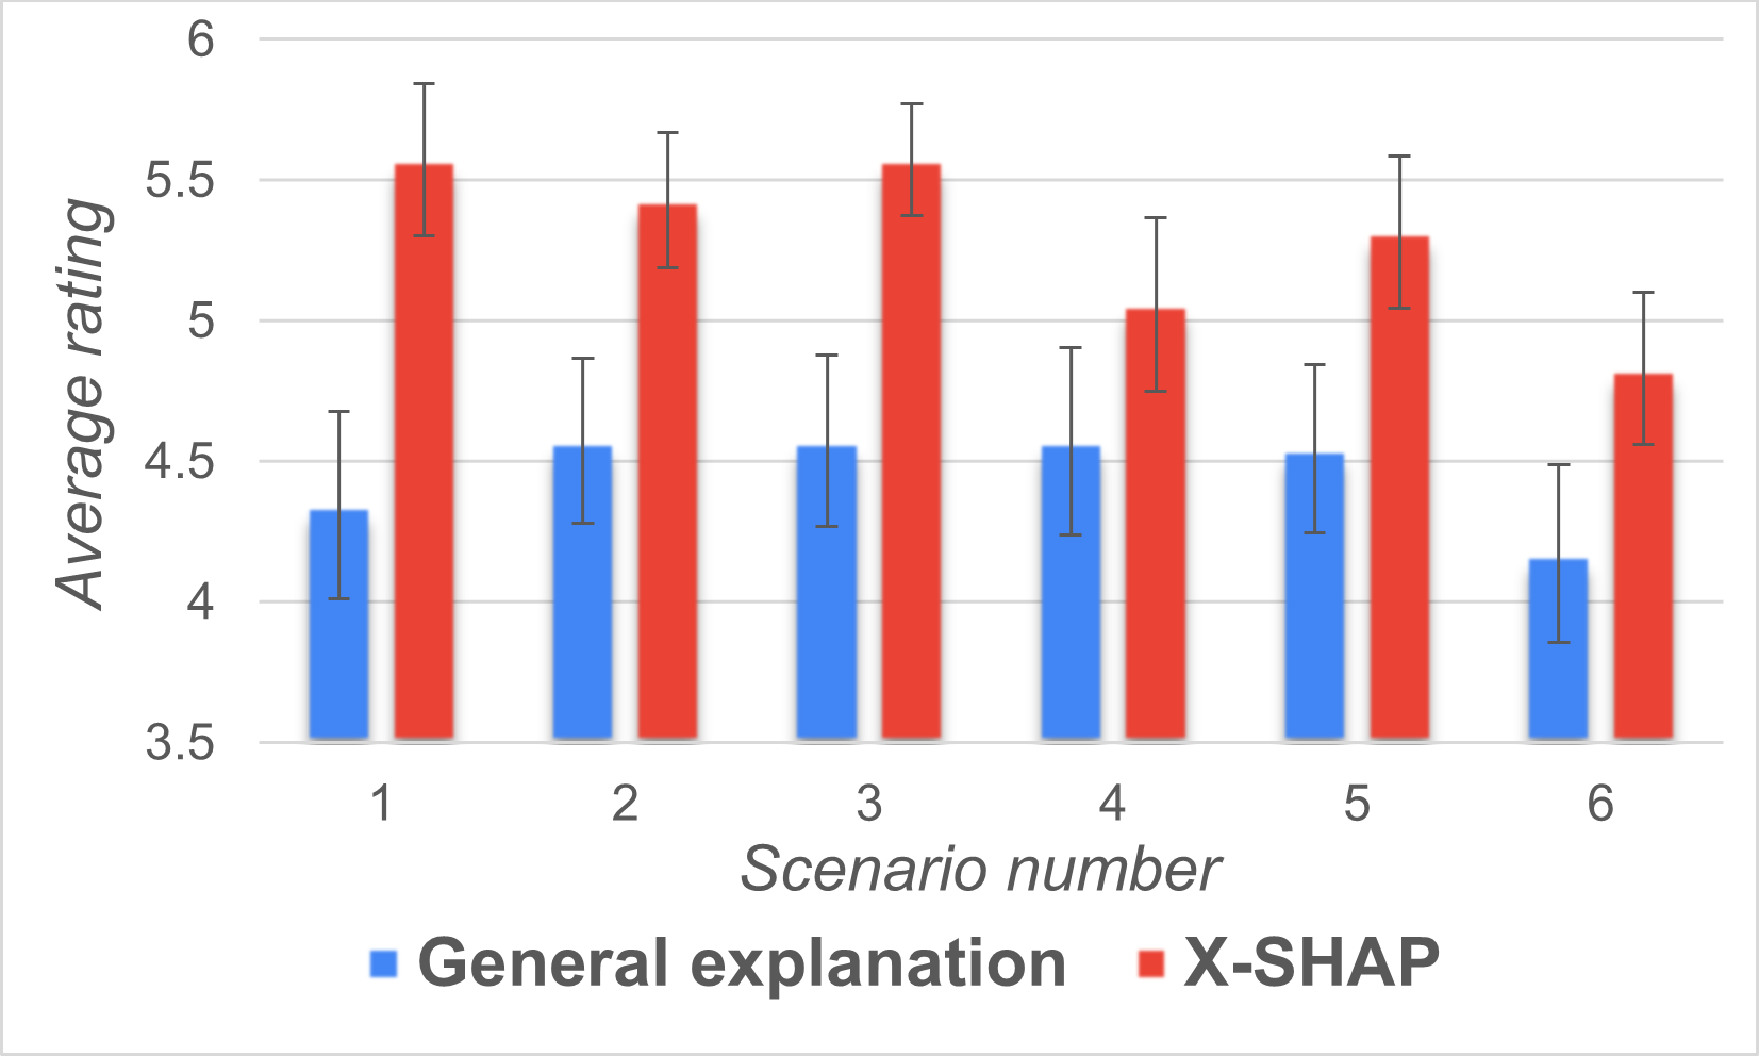
\includegraphics[width=3.3in]{ComparingResults.pdf}
%     \caption{Average rating of fairness for each of the two explanations in each of the six scenarios. Error bars present the standard error.}
%     \label{fig:comparingResult}
% \end{figure}



% \section{Conclusions and Future Work}
% The Shapley value is termed the most important normative division scheme in cooperative game theory. However, in some scenarios, its payoff allocation may seem unfair to humans. In this paper, we provided the first automatic method that generates customized explanations for the Shapley value. Our approach does not directly use psychological insights regarding the perception of fairness by humans. Instead, we utilize known mathematical axioms, and show that they can be used for increasing the rating of fairness of the Shapley allocation.
%We first define ETX games, which represent common scenarios and their Shapley allocation is easy to understand. We then presented X-SHAP, an algorithm that decomposes any coalitional game into ETX sub-games and generates a brief verbal explanation to every sub-game. We showed that X-SHAP outperforms a general explanation, which is not customized to a specific scenario, in terms of fairness rating by human subjects.

 
% Recall that the number of sub-games that X-SHAP shows to the user depends on the scenario and the number of agents. Therefore, in games with many agents, X-SHAP may be required to present its users with hundreds of sub-games, each game consisting of all subsets of the agents. 
% In future work, we intend to address this issue and propose three different complementary approaches.
% First, instead of presenting all the coalitions of a sub-game, X-SHAP can alternatively state that a specific coalition and any coalition containing it receive some payoff. 
% Furthermore, instead of presenting all sub-games, X-SHAP can present for a user only the sub-games in which she receives a non-zero payoff. Moreover, X-SHAP can present the explanations in an interactive process,
% %as a ``zero knowledge" like process,
% in which a user is provided with evidences (i.e., sub-games) until she is convinced that the provided allocation is fair. 
% This interactive process requires presenting the stronger evidence earlier during the process; this raises several interesting questions related to human perception of fairness.
%Alternatively, the sub-games can be provided only upon requests from the user. That is, the user will ask to see all sub-games where the payoff for a specific agent or coalition is not zero.
% Furthermore, since the easy to explain sub-games are sparse, we can show only the non-zero coalitions. If there are many agents, 

%\clearpage 
\bibliography{shapley}
\end{document}